\section{Pianificazione}



Lo sviluppo del progetto è diviso nei seguenti periodi:
\begin{enumerate}
	\item Analisi dei requisiti;
	\item Progettazione architetturale;
	\item Progettazione di dettaglio e codifica;
	\item Validazione e collaudo.
\end{enumerate}
In ogni periodo sono raggruppate le attività da svolgere.
I periodi e le attività delle prime due fasi sono individuati con una maggiore precisione rispetto a quelli successivi. Questo è dovuto alla difficoltà nel prevedere le modalità e i tempi richiesti dalle fasi più remote del progetto.
Nei \glock{diagrammi di Gantt} le barre verdi indicano attività di verifica.

Oltre alle attività riportate di seguito, verranno svolte le attività accessorie consistenti nelle riunioni interne ed esterne e produzione dei relativi verbali. Queste attività coinvolgono tutti i componenti e tutti i ruoli attivi nel periodo. 

\subsection{Analisi dei requisiti (dal 2020-10-22 al 2021-01-17)}

\subsubsection{Ruoli attivi}
\begin{itemize}
	\item Responsabile;
	\item Amministratore;
	\item Analista;
	\item Verificatore.
\end{itemize}

\subsubsection{Periodi e attività}

\paragraph{Primo periodo (dal 2020-10-22 al 2020-11-09)}
Questo periodo comincia con la costituzione del gruppo di progetto. Serve dunque a porre le basi per una comunicazione e collaborazione efficace ed efficiente. Vi si svolgono inoltre attività di ricerca superficiale sui capitolati.

\begin{itemize}
	\item Configurazione degli strumenti collaborativi basilari: comprende la scelta e la configurazione dei mezzi per la comunicazione e il lavoro collaborativo;
	\item Analisi superficiale dei capitolati.
	
\end{itemize}

\paragraph{Secondo Periodo (dal 2020-11-10 al 2020-12-13)}
Gli obiettivi raggiunti in questo periodo sono il consolidamento degli strumenti di collaborazione e l'approfondimento dei capitolati.
\begin{itemize}
	\item Configurazione del \glock{repository}: questa attività comprende la creazione di un repository per la condivisione e il versionamento dei prodotti, ma anche la sua configurazione per la verifica automatica della loro validità;
	\item Raccolta di informazioni dai seminari: stesura di appunti sui seminari, da poter facilmente consultare quando necessario;
	\item Studio dei progetti degli anni passati: questa attività ha il fine di individuare gli errori più comuni e le tecniche da prendere come esempio;
	\item Bozza dello studio di fattibilità;
	\item Bozza delle norme di progetto.
\end{itemize}

\paragraph{Terzo Periodo (dal 2020-12-14 al 2020-01-08)}
Questo periodo segue la scelta del capitolato da affrontare. È dedicato alla sua analisi approfondita e alla stesura della documentazione. 
\begin{itemize}
	\item Stesura delle norme di progetto;
	\item Stesura dello studio di fattibilità;
	\item Stesura del piano di progetto;
	\item Analisi dei requisiti e stesura dell'omonimo documento;
	\item Stesura del piano di qualifica;
	\item Stesura del glossario;
	\item Stesura della lettera di presentazione;
	\item Aggiornamento consuntivo;
	\item Verifica della documentazione.
\end{itemize}

\paragraph{Quarto Periodo (dal 2020-01-09 al 2020-01-17)}
È l'ultimo periodo di analisi dei requisiti. Si concentra quindi sulla preparazione dell'esposizione dei prodotti dei tre periodi precedenti.
\begin{itemize}
	\item Preparazione dell'esposizione;
	\item Verifica dell'esposizione.
\end{itemize}


\begin{landscape}
	\begin{figure}[H]
		\centering
		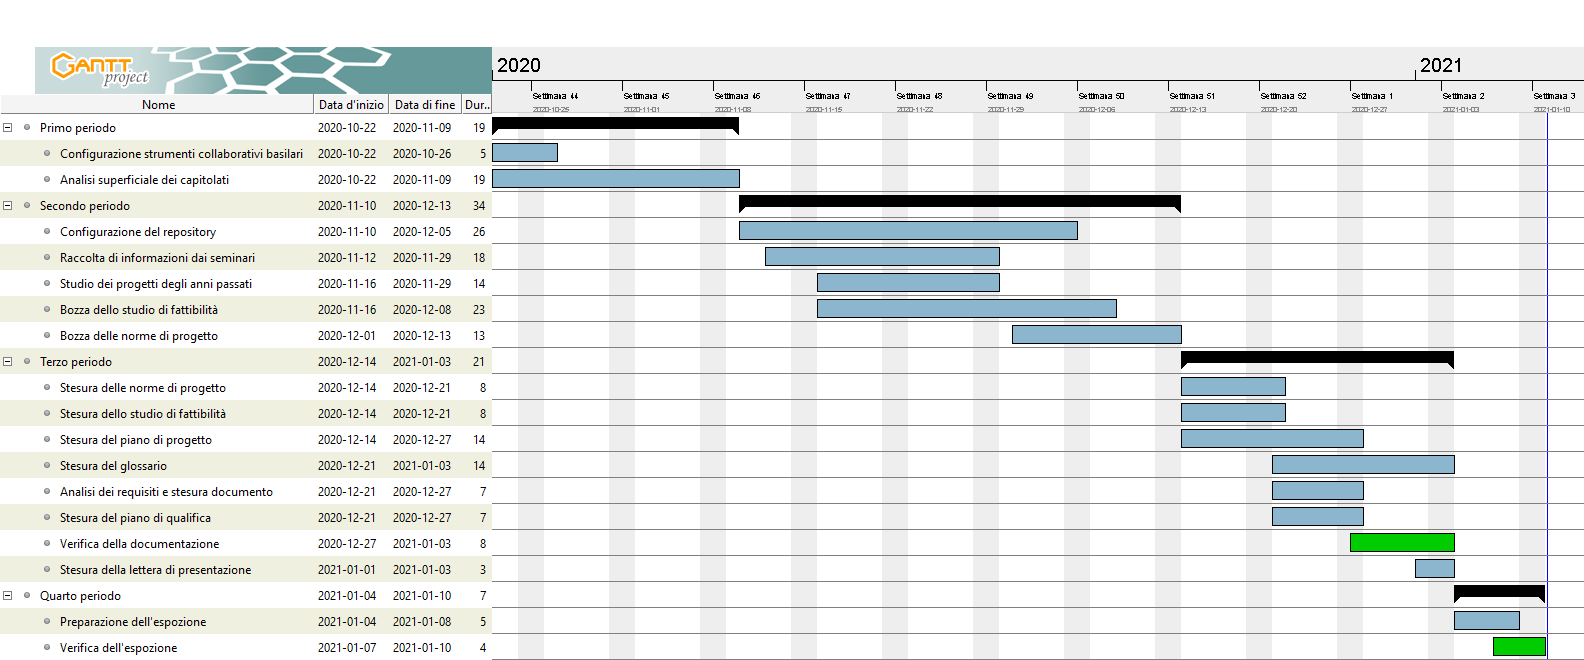
\includegraphics[width=\linewidth]{res/images/ganttFase1.png}
		\caption*{\textbf{Figura 1}{: Grafico di Gantt del periodo di analisi dei requisiti}}
		\label{fig:Gantt Analisi dei requisiti}
	\end{figure}
\end{landscape}




\subsection{Progettazione architetturale (dal 2021-01-18 al 2021-03-07)}

Questo periodo porta alla milestone della Revisione di Progettazione.
Durante questo periodo si vogliono individuare le tecnologie da utilizzare per lo sviluppo del prodotto e l'architettura su cui basarlo.
\subsubsection{Ruoli attivi}
\begin{itemize}
	\item Responsabile;
	\item Amministratore;
	\item Analista;
	\item Progettista;
	\item Verificatore.
\end{itemize}

\subsubsection{Attività da svolgere}
Sotto sono riportate le macro-attività da svolgere suddivise nelle rispettive attività:
\begin{enumerate}
	\item Aggiornamento PdQ
	\item Aggiornamento AdR
	\item Aggiornamento NdP
	\item Aggiornamento PdP
	\item Technology baseline
	\item Proof of concept
	\begin{enumerate}
		\item PoC Server
		\item PoC Ethereum
	\end{enumerate}
	\item Attività accessorie (produzione verbali, partecipazione a riunioni, etc...)
	\item Comunicazione con docenti
	\item Comunicazione con proponente
	\item Presentazione
\end{enumerate}

\subsubsection{Periodi}

\begin{figure}[H]
	\centering
	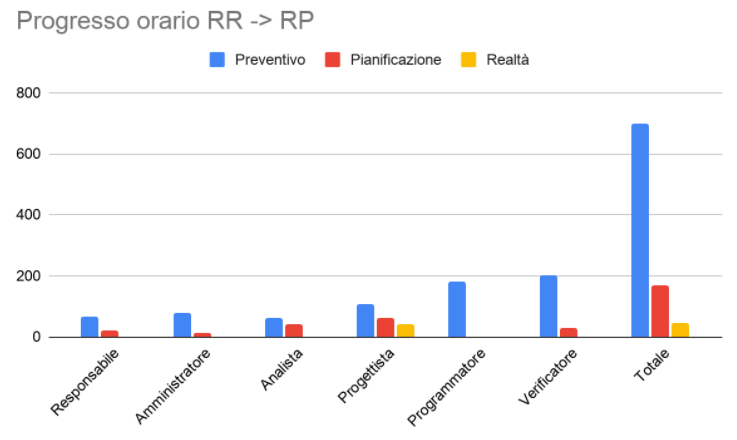
\includegraphics[width=0.7\linewidth]{res/images/scostamento2.1.png}
	\caption*{\textbf{Figura 6}: Scostamento}
	\label{fig:Figura2}
\end{figure}
\begin{figure}[H]
	\centering
	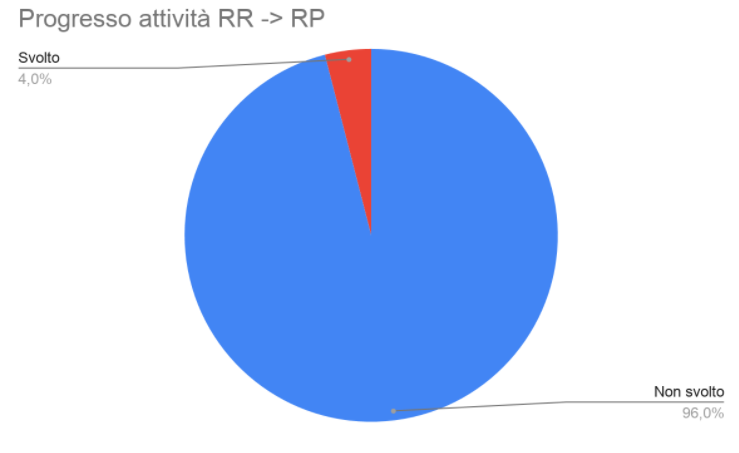
\includegraphics[width=0.7\linewidth]{res/images/completamento2.1.png}
	\caption*{\textbf{Figura 6}: Completamento}
	\label{fig:Figura2}
\end{figure}
\paragraph{Primo Periodo (15 febbraio)}
Per questo periodo è pianificato lo svolgimento delle seguenti attività suddivise tra rispettive macroattività:
	\begin{itemize}
		\item comunicazione docenti e proponenti
		\item Poc server
		\item Poc ethereum
	\end{itemize}


\begin{figure}[H]
	\centering
	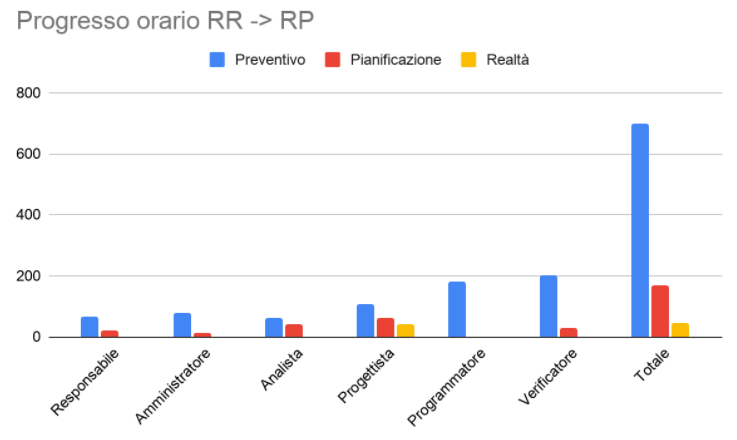
\includegraphics[width=0.7\linewidth]{res/images/scostamento2.1.png}
	\caption*{\textbf{Figura 6}: Scostamento}
	\label{fig:Figura2}
\end{figure}
\begin{figure}[H]
	\centering
	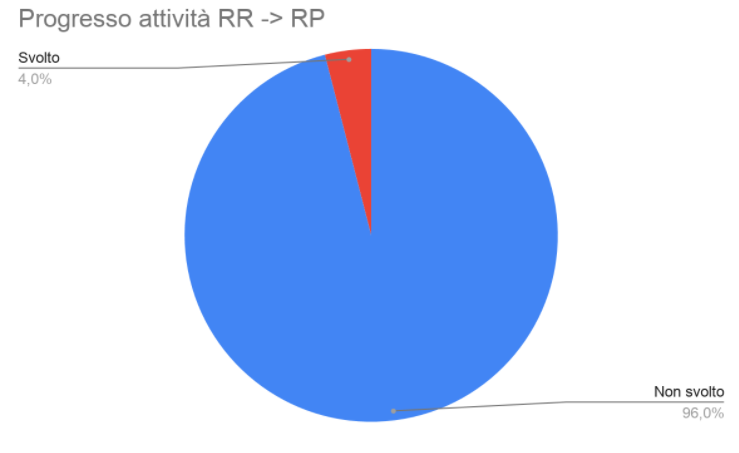
\includegraphics[width=0.7\linewidth]{res/images/completamento2.1.png}
	\caption*{\textbf{Figura 6}: Completamento}
	\label{fig:Figura2}
\end{figure}
\paragraph{Secondo Periodo (22 febbraio)}
Per questo periodo è pianificato lo svolgimento delle seguenti attività suddivise tra rispettive macroattività:
\begin{itemize}
	\item Poc server
	\item Poc ethereum
\end{itemize}





